% Mid-term report. Build: latexmk -pdf main.tex   (run inside report/)
% Layout follows "Report Format_midterm.docx" (Shiv Nadar University, Dept. of CSE):
% A4, Times New Roman 12pt, 1in side/bottom margins, ~1.15 Word line spacing,
% page numbers at the bottom centre, chapter-wise numbering of equations, figures
% and tables, IEEE references in order of appearance.
\documentclass[12pt,a4paper]{article}

\usepackage[utf8]{inputenc}
\usepackage[T1]{fontenc}
\usepackage{amsmath}
\usepackage{newtxtext,newtxmath}          % Times New Roman (template body font); provides amssymb symbols
\usepackage[a4paper,top=1in,bottom=1in,left=1in,right=1in,footskip=0.5in]{geometry}
\usepackage{setspace}
\setstretch{1.1}                          % ~ Word "Multiple 1.15" for Times 12pt
\usepackage{graphicx}
\usepackage{booktabs}
\usepackage{tabularx}
\usepackage{multirow}
\usepackage{xcolor}
\usepackage{tikz}
\usetikzlibrary{positioning,arrows.meta,fit}
\usepackage[numbers,sort&compress]{natbib}
\usepackage{tocloft}
\usepackage[hidelinks]{hyperref}
\usepackage{cleveref}

\graphicspath{{figures/}}
\newcommand{\todo}[1]{\textcolor{red}{[TODO: #1]}}

% Template: equations (2.1), figures and tables numbered per chapter (= section).
\numberwithin{equation}{section}
\numberwithin{figure}{section}
\numberwithin{table}{section}

% Front-matter page heading: centred, bold, 14pt (template "Declaration" style).
\newcommand{\frontheading}[1]{%
  \begin{center}{\fontsize{14}{17}\selectfont\bfseries #1\par}\end{center}
  \vspace{0.8em}}

% Contents / lists: centred headings in the same style, single-spaced entries.
\renewcommand{\cfttoctitlefont}{\hspace*{\fill}\fontsize{14}{17}\selectfont\bfseries}
\renewcommand{\cftaftertoctitle}{\hspace*{\fill}}
\renewcommand{\cftloftitlefont}{\hspace*{\fill}\fontsize{14}{17}\selectfont\bfseries}
\renewcommand{\cftafterloftitle}{\hspace*{\fill}}
\renewcommand{\cftlottitlefont}{\hspace*{\fill}\fontsize{14}{17}\selectfont\bfseries}
\renewcommand{\cftafterlottitle}{\hspace*{\fill}}
\setlength{\cftbeforetoctitleskip}{0pt}
\setlength{\cftbeforeloftitleskip}{0pt}
\setlength{\cftbeforelottitleskip}{1.5em}
\setlength{\cftfignumwidth}{2.8em}
\setlength{\cfttabnumwidth}{2.8em}
\setcounter{tocdepth}{2}

\begin{document}

% ---------------- front matter: title (unnumbered), then i, ii, ... ----------
% Title page. Wording, order and point sizes follow "Report Format_midterm.docx"
% (title 24pt; degree lines 22pt bold; "Submitted by" 16pt italic; names 16pt;
% supervision block 18pt; month/year 14pt). Unnumbered.
\begin{titlepage}
\centering
\singlespacing

{\fontsize{24}{29}\selectfont Structure--Content Disagreement for Community-Aware
 Misinformation Containment\par}
\vspace{0.4cm}
{\fontsize{14}{17}\selectfont Mid-Term Report\par}
\vfill

{\fontsize{14}{17}\selectfont Project Report Submitted in Partial Fulfilment of the
 Requirements for the Degree of\par}
\vfill

{\fontsize{22}{26}\selectfont\bfseries Bachelor of Technology\par}
\vspace{0.2cm}
{\fontsize{22}{26}\selectfont\bfseries\itshape in\par}
\vspace{0.2cm}
{\fontsize{22}{26}\selectfont\bfseries Computer Science and Engineering\par}
\vfill

{\fontsize{16}{19}\selectfont\itshape Submitted by\par}
\vspace{0.3cm}
{\fontsize{16}{20}\selectfont
 Abhyudaya Vasisht (Roll No. 2410111184)\par
 Shruti Sharma (Roll No. 2310110715)\par}
\vfill

{\fontsize{18}{22}\selectfont\bfseries\itshape Under the Supervision of\par}
\vspace{0.3cm}
{\fontsize{18}{22}\selectfont Dr.\ Suchi Kumari\par}
\vfill


\includegraphics[width=3.6cm]{00_front_matter/snu_logo.jpeg}\par
\vspace{0.1cm}

{\fontsize{18}{22}\selectfont Department of Computer Science and Engineering\par}
\vspace{0.3cm}
{\fontsize{14}{17}\selectfont October, 2026\par}

\vspace*{0.5cm}
\end{titlepage}


\pagenumbering{roman}
\setcounter{page}{1}
% Declaration. Text is verbatim from "Report Format_midterm.docx"; the template asks
% for "Name of the Student ____ Signature and Date ____" for all members of the group.
\frontheading{Declaration}

I/We declare that this written submission represents my ideas in my own words and
where others' ideas or words have been included, I have adequately cited and
referenced the original sources. I also declare that I have adhered to all
principles of academic honesty and integrity and have not misrepresented or
fabricated or falsified any idea/data/fact/source in my submission. I understand
that any violation of the above will be cause for disciplinary action by the
University and can also evoke penal action from the sources which have thus not been
properly cited or from whom proper permission has not been taken when needed.

\vspace{2cm}
\noindent\textbf{Name of the Student:} Abhyudaya Vasisht (Roll No. 2410111184)\par
\vspace{1.5cm}
\noindent\textbf{Signature and Date:} \rule{6cm}{0.4pt}\par
\vspace{1.5cm}
\noindent\textbf{Name of the Student:} Shruti Sharma (Roll No. 2310110715)\par
\vspace{1.5cm}
\noindent\textbf{Signature and Date:} \rule{6cm}{0.4pt}\par

\clearpage

\frontheading{Abstract}
Misinformation spreads inside groups of people who are both connected and like-minded,
and crosses into other groups through a small number of accounts and links. Most
containment methods choose where to intervene from network structure alone. This
project asks whether a second signal, the content a user posts, can identify
intervention targets that structure misses. We define, for every user, a
\emph{structural} community membership (from the social graph) and a \emph{content}
membership (what a classifier that reads only the user's text predicts that community
to be), and score the disagreement between the two. The classifier receives no edges
or graph-derived features as input; the graph communities are used only as its
training targets. The idea comes from
the use of complementary clusterings to locate ambiguous regions in active
learning~\citep{sani2026aas}. This mid-term report describes the motivation, related
work, the methodology as currently built, and the experimental setup on two real
social networks (TIMME political Twitter and the Pokec social network) and on
controlled synthetic networks, together with the current status and the plan for the
rest of the project. Results are not reported here.

\clearpage

{\singlespacing
\tableofcontents
\clearpage
\listoffigures
\listoftables
\clearpage}

% ---------------- main text: arabic, restarting at 1 ------------------------
\pagenumbering{arabic}
\setcounter{page}{1}

\section{Introduction}
\label{sec:intro}

\subsection{Motivation}
Online social networks are organised into communities: groups of users who can reach
one another easily and who tend to share views and interests. A false message usually
starts inside one such group. Its reach depends largely on whether it crosses into
other groups, and that crossing happens through comparatively few accounts and links
that connect otherwise separate parts of the network~\citep{shah2024telegram}.
Intervening at those crossings, by removing, throttling or labelling the content that
passes through them, is the premise behind community-aware misinformation
containment~\citep{ghoshal2021community}.

The standard way to choose where to intervene is structural. Influence blocking
methods rank nodes by degree, PageRank, betweenness or bridging scores computed from
the graph alone~\citep{budak2011limiting,xie2025blocking}. Structure, however, only
says who is connected to whom. It does not say who is likely to \emph{accept} a
message. A user whose friends are all in one community but who writes like members of
another is structurally ordinary and invisible to these scores, yet may be exactly the
point where a message from that other community gets in.

\subsection{Idea}
The project builds two separate views of the same users:
\begin{itemize}
  \item a \textbf{topology view}, in which communities are found from the social graph
        alone; and
  \item a \textbf{content view}, in which a classifier that reads only each user's own
        text predicts which of those communities the user belongs to.
\end{itemize}
The content view receives no edges or graph-derived features as input; the topology
communities are used only as its training targets. Where the two views agree, the two
sources of evidence about the user are consistent, although both could still be wrong.
Where they disagree, the user's edges say one thing and their words say another. We call this
\emph{structure--content disagreement} and score it per node.

The idea follows the Ambiguity-Aware Sampling (AAS) framework of
\citet{sani2026aas}, which runs two complementary clustering methods on the same data
and treats the regions where they disagree as the most informative places to spend
an annotation budget. We carry that principle from image embeddings to social
networks. Our two views are structure and content, not two clustering algorithms on
one embedding. The question is whether the disagreement points to useful intervention
targets.

\subsection{Objectives}
\begin{enumerate}
  \item Build a topology view and a content view, where the content view takes no
        edges or graph-derived features as input and uses the topology communities
        only as cross-fitted training targets, and a per-node disagreement score
        between them.
  \item Test whether the score detects nodes whose content and structure genuinely
        conflict, on synthetic networks with planted conflicts and on a real network
        with party labels (TIMME).
  \item Test, by simulating spread with an unknown source, whether targeting nodes
        or links with high disagreement contains spread better than strong
        structural baselines, and map the conditions under which it does.
  \item (Planned extension) Use the disagreement to choose queries in an active
        learning loop, as in AAS.
\end{enumerate}

\subsection{Scope of this report}
This is a mid-term report. It covers the problem, prior work, the methodology as
implemented, the experimental setup, and the status and plan of the work.
Experimental results are deliberately left out and will be reported in the final
report.

\subsection{Organisation}
\Cref{sec:related} reviews related work and explains how it led to the current idea.
\Cref{sec:method} describes the methodology and its limitations. \Cref{sec:setup}
describes the datasets, parameters, baselines and evaluation measures.
\Cref{sec:status} summarises what has been built and what remains.

\section{Related Work}
\label{sec:related}

\subsection{Community structure in social networks}
Community detection partitions a graph into groups that are densely connected inside
and sparsely connected to each other. The usual quality measure is
modularity~\citep{newman2006modularity}, which compares the share of edges inside
communities with the share expected in a random graph that has the same degrees. The
Louvain method~\citep{blondel2008louvain} optimises modularity greedily. Leiden
\citep{traag2019leiden} refines it and guarantees that every community is connected;
we use Leiden. Detection algorithms always return a partition, even on random graphs,
so it is standard to compare against a degree-preserving randomised
graph~\citep{maslov2002specificity}. Separate runs of the same stochastic algorithm
also disagree, and \citet{riolo2020consistency} use that run-to-run variation to
measure how consistently each node is assigned. We use it as a structure-only
baseline.

\subsection{Node metadata versus network structure}
Users carry metadata (biographies, posts, declared interests) alongside their edges.
\citet{newman2016annotated} show that metadata and structural communities can agree
or disagree, and that how well the metadata predicts the community is itself
informative. This is the closest precedent for our content view, which asks what
community a node's text predicts. Community outlier detection~\citep{gao2010outliers}
flags nodes whose attributes are far from the rest of their community. We use a simple
version of that idea (distance from the community's text centroid) as a baseline.

\subsection{Bridges and ambiguous membership}
Several lines of work suggest that nodes between communities matter more for spreading
than their degree implies. The participation coefficient of
\citet{guimera2005functional} measures how evenly a node's links are spread across
communities. \citet{nepusz2008fuzzy} define \emph{bridgeness} from fuzzy (soft)
community memberships, so a node with ambiguous membership is a bridge. In epidemic
models on community-structured networks, \citet{salathe2010dynamics} found that
immunising community bridges can beat immunising high-degree nodes when community
structure is strong. On Telegram, \citet{shah2024telegram} identified channels that
connect misinformation communities and proposed them as intervention targets. All of
these define bridges or ambiguity from structure alone.

\subsection{Spread models and influence blocking}
The Independent Cascade (IC) model~\citep{kempe2003maximizing} spreads a message along
each edge independently with some probability. Its \emph{weighted cascade} variant
sets that probability to $1/\deg(v)$ for the receiving node $v$. Influence Blocking
Maximization (IBM) chooses nodes or links to block so that a harmful cascade
reaches as few users as possible~\citep{budak2011limiting}. The problem is NP-hard, and
unlike influence maximisation its objective is not supermodular, so greedy algorithms
come with no general approximation guarantee~\citep{xie2025blocking}. Community-aware
variants choose blockers using the community partition~\citep{ghoshal2021community}.
Most IBM work assumes the source of the misinformation is known; \citet{chen2021uncertain}
treat the source as uncertain, which is the setting we adopt. Strong structural
baselines include PageRank, betweenness, adaptive degree and Collective
Influence~\citep{morone2015influence}. Which of these wins depends on how easily the
message is transmitted~\citep{hebert2013global}, so we sweep the transmission
probability rather than fix one value.

Spread on real platforms also depends on content. \citet{delvicario2016spreading}
document selective exposure: users mostly share content that agrees with their
group's views. This motivates our content-aware spread model, in which the chance of
passing a message on depends on how closely the receiver's content matches the
community the message came from.

\subsection{Self-supervised graph embeddings}
The original plan was to embed every node from text and topology together using
self-supervised graph neural networks, then cluster the embedding. We trained three
objective families on a shared encoder: BGRL (bootstrapping, no
negatives)~\citep{thakoor2022bgrl}, Deep Graph Infomax (mutual
information)~\citep{velickovic2019dgi} and MVGRL (adjacency view against diffusion
view)~\citep{hassani2020mvgrl}. \Cref{sec:method-evolution} explains why this design
was replaced.

\subsection{Active learning with clustering ambiguity}
In graph active learning, AGE~\citep{cai2017age} picks nodes to label by combining
prediction entropy, centrality and distance to cluster centres. So ``uncertainty plus
centrality'' is already an established design, though its uncertainty is about a
node's \emph{class label}. AAS~\citep{sani2026aas}, built for animal
re-identification, takes a different route. It runs two complementary clusterings
(density-based and nearest-neighbour) on the same embedding, builds an overlap graph
between their clusters, and treats connected regions of partial overlap as
\emph{ambiguous regions}. It then samples must-link and cannot-link pair queries from
those regions and refines the clustering with the oracle's answers. AAS is the
starting point of this project.

\subsection{From related work to the current idea}
\label{sec:related-gap}
Three observations shaped the current design.
\begin{enumerate}
  \item \textbf{Both halves of the original idea already exist.} Community-aware
        blocking~\citep{ghoshal2021community} and uncertainty combined with
        centrality~\citep{cai2017age} are both published. A defensible contribution has
        to be narrower.
  \item \textbf{Existing ambiguity is structural.} Bridgeness, participation and
        consensus ambiguity~\citep{nepusz2008fuzzy,guimera2005functional,riolo2020consistency}
        are all computed from the graph. None of them can see a node whose edges place
        it in one community and whose content places it in another.
  \item \textbf{AAS-style disagreement needs separate views.} Two clusterings of
        one embedding disagree partly because of the algorithms themselves. If one
        view is derived from the other (for example, a content clustering built from a
        graph embedding), their disagreement cannot be read as a property of the node.
\end{enumerate}
We therefore keep the AAS principle (look where complementary views disagree) and
keep the inputs of the two views separate: topology from edges only, content from text
only. The separation is in the inputs, not complete: the content classifier is trained
to predict the topology communities, so its targets come from the graph. It never
receives edges or graph-derived features, and cross-fitting ensures that no node's own
label informs its prediction. The working claim is that \emph{metadata-aware membership ambiguity}
identifies containment targets that purely structural bridge and centrality scores
miss, and the experiments are designed to find out when, if ever, that claim holds.

\section{Methodology}
\label{sec:method}

\Cref{fig:pipeline} shows the pipeline. It has two separate views of the same
users (\cref{sec:method-views}), per-node membership vectors and disagreement scores
(\cref{sec:method-scores}), a detection check (\cref{sec:method-detect}) and a spread
simulation that tests interventions (\cref{sec:method-block}).

\begin{figure}[t]
\centering
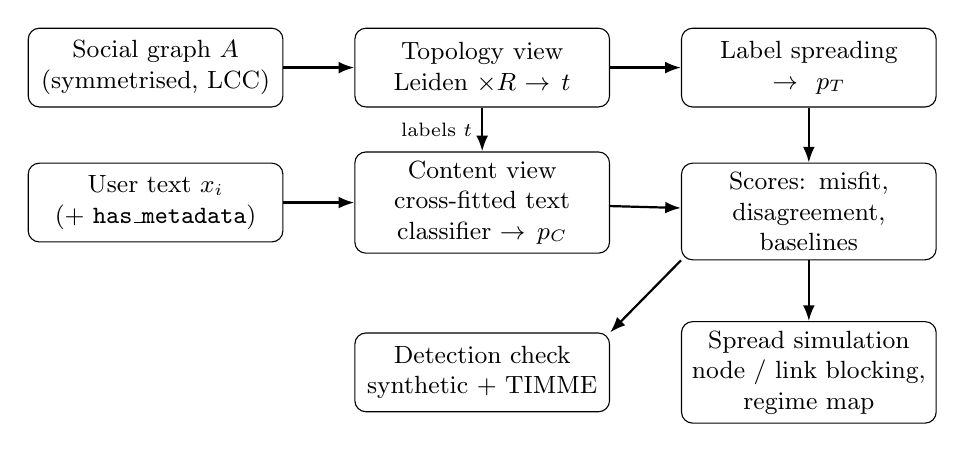
\begin{tikzpicture}[
  box/.style={draw, rounded corners, align=center, minimum height=1.0cm,
              text width=3.0cm, font=\small},
  arr/.style={-{Latex[length=2mm]}, thick},
  node distance=0.7cm and 0.9cm]
  \node[box] (graph) {Social graph $A$\\(symmetrised, LCC)};
  \node[box, below=of graph] (text) {User text $x_i$\\(+ \texttt{has\_metadata})};

  \node[box, right=of graph] (leiden) {Topology view\\Leiden $\times R$ $\to t$};
  \node[box, right=of text] (clf) {Content view\\cross-fitted text\\classifier $\to p_C$};

  \node[box, right=of leiden] (spread) {Label spreading\\$\to p_T$};
  \node[box, below=of spread] (scores) {Scores: misfit,\\disagreement, baselines};

  \node[box, below=1.0cm of clf] (detect) {Detection check\\synthetic + TIMME};
  \node[box, right=of detect] (block) {Spread simulation\\node / link blocking,\\regime map};

  \draw[arr] (graph) -- (leiden);
  \draw[arr] (text) -- (clf);
  \draw[arr] (leiden) -- (spread);
  \draw[arr] (leiden) -- node[left, font=\scriptsize] {labels $t$} (clf);
  \draw[arr] (spread) -- (scores);
  \draw[arr] (clf) -- (scores);
  \draw[arr] (scores) -- (block);
  \draw[arr] (scores.south west) -- (detect.north east);
\end{tikzpicture}
\caption{Pipeline. The topology view uses edges only. The content view receives no
edges or graph-derived features as input; the topology labels $t$ are used only as
its training targets, with cross-fitting so that no node's own label informs its
prediction.}
\label{fig:pipeline}
\end{figure}


\subsection{Problem formulation}
\label{sec:method-problem}
Let $G=(V,E)$ be a social graph with $n=|V|$ users and adjacency matrix $A$. Every
user $i$ has a text vector $x_i$ (\cref{sec:setup-features}), which is zero if the
user has no text. We treat ties as undirected (requirement R5,
\cref{sec:setup-requirements}). The aim is to:
\begin{enumerate}
  \item assign every user a structural community $t_i \in \{1,\dots,K\}$ from $A$ alone;
  \item estimate two soft memberships over those $K$ communities, a structural one
        $p_T(i)$ and a content one $p_C(i)$, where $p_C(i)$ depends only on text;
  \item score how far apart they are; and
  \item decide whether blocking high-scoring nodes or links reduces spread from an
        \emph{unknown} source more than structural targeting does, for a fixed budget.
\end{enumerate}

\subsection{Design evolution}
\label{sec:method-evolution}
The first design followed AAS closely. Each node would be embedded from text and
topology together with a self-supervised GNN (BGRL, DGI or MVGRL on a shared two-layer
GCN encoder), and the embedding would be clustered by a density method (HDBSCAN) and a
first-neighbour method (FINCH). Ambiguous regions would come from where those two
clusterings partly overlap. Diagnostics during development showed that the clusters of
these embeddings mainly sorted nodes by degree rather than by community
(\cref{tab:gnn-diag}). On TIMME, for all three objectives, the two-way $k$-means split
of the embedding and its first principal component were both strongly correlated with
log-degree, while the six-way $k$-means partition had negative modularity on the
social graph and almost no mutual information with party. Party information was not
missing from the embeddings: a linear probe predicted party well above the majority
baseline. It was present, but the cluster structure followed degree, not communities.
These numbers are a development diagnostic of the discarded design, shown only because
they motivated the redesign. There was also a design flaw: a content view derived from
an embedding that has already seen the graph cannot disagree with the graph in a
meaningful way. The GNN stage was therefore replaced by the two separate views below. The AAS principle of looking where
complementary views disagree is kept.

\begin{table}[t]
\centering
\caption{Development diagnostic of the discarded GNN design on TIMME (20,811 nodes,
1,206 with party labels). Clusters are $k$-means on L2-normalised embeddings. Shown
only to justify the redesign (\cref{sec:method-evolution}); these are not results of
the current pipeline.}
\label{tab:gnn-diag}
\small
\begin{tabular}{@{}l r r r@{}}
\toprule
Diagnostic & BGRL & DGI & MVGRL \\
\midrule
$|r|$, $k=2$ split vs.\ log-degree           & 0.58   & 0.60   & 0.67   \\
$|r|$, first principal component vs.\ log-degree & 0.66 & 0.70  & 0.78   \\
Modularity of the $k=6$ partition            & $-0.050$ & $-0.152$ & $-0.104$ \\
Party NMI of the $k=6$ partition             & 0.060  & 0.018  & 0.002  \\
Linear party probe accuracy (5-fold)$^{*}$   & 0.943  & 0.934  & 0.780  \\
\bottomrule
\end{tabular}

\smallskip
\footnotesize
$^{*}$Logistic regression on the embedding, labelled users only; always predicting
the majority party gives 0.534.
\end{table}


\subsection{Preprocessing}
\label{sec:method-pre}
For every dataset we remove self-loops, make every edge two-way and keep the
\emph{largest connected component} (a node with no path to the rest of the network
cannot pass a message on). Users without text are \emph{kept}, because removing them
would also remove their edges, and some of those edges may be bridges. Such users get
a zero text vector and a binary \texttt{has\_metadata} flag.

\subsection{Two separate views}
\label{sec:method-views}

\paragraph{Topology view.}
Leiden~\citep{traag2019leiden} with the modularity objective is run on $G$ with $R$
different random seeds. The run with the highest modularity is the reference partition
$t$. Communities containing fewer than 1\% of the nodes are set aside ($t_i=-1$): they
are never used as training targets or as seeds for spreading. The remaining $K$
communities form the label space. All $R$ runs are kept for the consensus baseline.

\paragraph{Content view.}
Content membership is estimated with \emph{cross-fitting}. The users with $t_i \ge 0$
are divided into $F$ stratified folds. For each fold, a multinomial logistic
regression (with standardised inputs and $L_2$ regularisation) is trained on the other
folds to predict $t$ from the text vector $x$, and is then applied to the held-out
fold. The result is
\begin{equation}
  p_C(i) = \Pr\bigl(t_i = \cdot \mid x_i\bigr) \in \Delta^{K-1},
\end{equation}
where every $p_C(i)$ comes from a model that never saw user $i$'s own label. Users with
$t_i=-1$ are scored by every fold model and the predictions are averaged. The
classifier receives no edges or graph-derived features as input; the topology labels
$t$ are used only as training targets, with cross-fitting so that no node's own label
informs its prediction. The two views are therefore separate in their inputs, but not
fully independent: the content view learns which text goes with which graph
community.

\paragraph{Structural soft membership.}
The hard partition $t$ is turned into soft memberships by label
spreading~\citep{zhou2004learning}. With $Y$ the one-hot matrix of $t$ (zero rows for
$t_i=-1$) and $S = D^{-1/2} A D^{-1/2}$,
\begin{equation}
  F^{(m+1)} = \alpha\, S F^{(m)} + (1-\alpha)\, Y, \qquad F^{(0)} = Y,
\end{equation}
iterated a fixed number of times. Each row is then normalised to give $p_T(i)$. Users
deep inside a community end up with an almost one-hot $p_T(i)$; users on a boundary
end up with mixed rows.

\subsection{Per-node scores}
\label{sec:method-scores}
Three scores use the two views:
\begin{align}
  \text{misfit}_i &= 1 - p_C(i)_{t_i}, \\
  \text{disagreement}_i &= \mathrm{JS}_2\bigl(p_T(i)\,\Vert\,p_C(i)\bigr), \\
  \text{ambiguity}^T_i &= H\bigl(p_T(i)\bigr) / \log K.
\end{align}
Misfit measures how little the text supports the node's own community.
Disagreement is the base-2 Jensen--Shannon divergence~\citep{lin1991divergence}
between the two memberships, which lies in $[0,1]$. Structural ambiguity is the
normalised entropy of the structural membership and uses no text.
For $t_i=-1$, misfit is defined as $1-\max_k p_C(i)_k$.

\paragraph{Baselines.}
These are the scores the proposed ones have to beat. Each captures one alternative
explanation of what disagreement might be measuring:
\begin{itemize}
  \item \textbf{Consensus entropy} (structure only): every Leiden run is aligned to $t$
        with the Hungarian algorithm, and the score is the normalised entropy of each
        node's label across runs~\citep{riolo2020consistency}.
  \item \textbf{Participation coefficient}~\citep{guimera2005functional}:
        $P_i = 1-\sum_c (h_{ic}/d_i)^2$, where $h_{ic}$ is the number of $i$'s
        neighbours in community $c$ and $d_i$ is $i$'s degree.
  \item \textbf{Content outlier}, following \citet{gao2010outliers}:
        $1-\cos(x_i, \bar{x}_{t_i})$, the cosine distance from the centroid of the
        node's community's text.
  \item \textbf{Degree} and \textbf{PageRank}, to check that a score is not simply
        degree in disguise.
\end{itemize}

\subsection{Checking that the scores detect real conflicts}
\label{sec:method-detect}

\paragraph{Synthetic benchmark with planted conflicts.}
Synthetic networks have a known answer. The generator is a degree-corrected block
model in the style of LFR~\citep{lancichinetti2008benchmark,karrer2011stochastic}.
Degrees follow a power law. A share $\mu$ of each node's edge stubs is matched across
communities (the mixing parameter), and the rest is matched inside the node's own
community. Each node's text is its community's centroid plus Gaussian noise of scale
$\sigma$, normalised to unit length. A small share of nodes is \emph{planted}: they
get the text centroid of a different community, and these are the true conflicts.
Real text also varies for reasons that have nothing to do with community, so an
optional \emph{nuisance} block adds random topics and a writing-style direction
proportional to log-degree. The full pipeline (Leiden, cross-fitted classifier,
scores) is run on each network. Every score is evaluated by ROC AUC for recovering
the planted nodes, both overall and within degree terciles (so a score cannot win
just by tracking degree).

\paragraph{Real-data check on TIMME.}
TIMME has party labels for part of the users (\cref{sec:setup-data}). A labelled user
counts as a \emph{party misfit} when their party differs from the majority party of
their topology community. Only communities with at least 20 labelled users and at
least 80\% one party are used, because a mixed community has no ``wrong'' side. Each
score is evaluated by AUC for predicting party misfits, overall and within degree
terciles, with a one-sided Mann--Whitney test. As a null, the text rows are shuffled
across users and all scores are recomputed. A real score has to beat its own
shuffled-text version.

\subsection{Testing interventions with spread simulation}
\label{sec:method-block}

\paragraph{Spread model.}
We use live-edge Independent Cascade~\citep{kempe2003maximizing}. An edge $u\to v$
transmits with probability $p_{uv}$ under one of two schemes:
\begin{itemize}
  \item \emph{weighted cascade}, $p_{uv}=1/\deg(v)$;
  \item \emph{uniform}, $p_{uv}=c\cdot p_c$, where
        $p_c = \langle k\rangle / (\langle k^2\rangle - \langle k\rangle)$ is the
        epidemic threshold of a network with this degree
        sequence~\citep{newman2002spread}, and $c$ is swept over several multiples.
\end{itemize}

\paragraph{Unknown source and common random numbers.}
In every simulation the seeds are drawn uniformly from nodes that \emph{no} strategy
blocks at the largest budget, so no strategy can win by deleting the source. Every
strategy and budget sees the same live-edge samples and the same seeds (common random
numbers), so differences between strategies are not Monte Carlo noise.

\paragraph{Outcomes.}
For each run we record the \emph{infected share} (seeds excluded) and the
\emph{cross-community share}, i.e.\ infected users outside every seed's community.
Each strategy is reported as the percentage of spread it removes compared with no
blocking.

\paragraph{Content-aware spread.}
Under selective exposure~\citep{delvicario2016spreading} a message is accepted more
readily by users whose content matches the community it came from. Each cascade
starts in one community $A$ (seeds drawn inside $A$), and every edge probability is
reweighted:
\begin{equation}
  p'_{uv} = \min\bigl(1,\; p_{uv}\cdot K\cdot a_v(A)\bigr),
\end{equation}
where $a_v \in \Delta^{K-1}$ is node $v$'s affinity to each community's content. The
multiplier $K\,a_v(A)$ averages approximately 1 over receivers, so the overall
transmission rate stays roughly the same. This is only approximate: the affinities
average exactly $1/K$ across receivers only when the communities are of equal size,
and the $\min(1,\cdot)$ clipping lowers the effective rate further. On
TIMME, $a_v$ comes from a separate cross-fitted classifier trained on a \emph{different}
text source (GloVe tweet averages) from the one used for scoring (MiniLM). This keeps
the spread model from reusing the scorer's own predictions.

\paragraph{Node-blocking strategies.}
Given a budget $k$, each strategy removes its top-$k$ nodes. Structural strategies:
random, degree, adaptive degree (recomputed after each removal), PageRank, sampled
betweenness, Collective Influence at radius 1~\citep{morone2015influence},
participation coefficient, and participation, consensus entropy and structural
ambiguity each multiplied by PageRank. Content-based strategies: misfit,
disagreement, content outlier (alone and multiplied by PageRank), and a
\emph{gateway} score
\begin{equation}
  g_i = \sum_{A} h_{iA}\; a_i(A)\; \bigl(d_i - h_{iA}\bigr),
\end{equation}
which estimates how much of community $A$'s content node $i$ can carry out of $A$.
In words: for each community $A$, the number of $i$'s neighbours in $A$, weighted by
how well $i$'s content matches $A$, is multiplied by the number of $i$'s neighbours
outside $A$, and these products are summed over communities. The
same formula with $a_i(A)=1/K$ (``structural gateway'') removes the text, so comparing
the two isolates what the content adds.

\paragraph{Link-level intervention.}
Instead of removing accounts, we can add friction to individual links (both directions
of an undirected link are cut together). Link scores: random, degree product, PageRank
product, a structural bridge score (cross-community links ranked by
$\mathrm{PR}_u\mathrm{PR}_v$), and two content-aware variants. The first ranks
cross-community links by
$\max\bigl(\mathrm{PR}_u\, p_C(v)_{t_u},\ \mathrm{PR}_v\, p_C(u)_{t_v}\bigr)$, i.e.\ an
influential sender times a receptive receiver. The second multiplies the structural
bridge score by that receptivity.

\paragraph{Regime map.}
Real networks fix the community strength and the size of the content effect, so a
single dataset cannot show when content-aware targeting helps. We therefore sweep
these factors on synthetic networks:
\begin{itemize}
  \item the mixing $\mu$;
  \item the agreement effect $\beta$, which sets the affinity
        $a_v(A) \propto \exp\bigl(\beta\,[c_v = A]\bigr)$ for node $v$'s \emph{true}
        content community $c_v$ ($\beta=0$ is content-blind spread);
  \item the share of mismatched nodes; and
  \item where the mismatched nodes are placed: uniformly at random, or in proportion
        to degree (``hub'').
\end{itemize}
Scores are computed from \emph{observed}, noisy text through the full pipeline, while
spread uses the true content. For each setting we report the paired gain, in
cross-community spread removed, of each content-aware strategy over the better of
PageRank and betweenness, with a 95\% confidence interval.

\subsection{Planned extension: active learning}
\label{sec:method-al}
AAS uses disagreement to choose must-link and cannot-link pair queries for an oracle
and then refines the clustering under those constraints. A version of that loop, with
queries drawn from high-disagreement nodes and a simulated oracle built from TIMME
party labels, is planned as an extension and depends on discussion with the
supervisor. It is not part of the work described in this report.

\subsection{Limitations}
\label{sec:method-limits}
Three limitations of the design are known in advance.
\begin{itemize}
  \item \textbf{Content-aware spread may favour content scores by construction.} The
        receiver affinity $a_v$ is itself a text-to-community classifier trained on
        the same topology labels $t$. Strategies that use $p_C$ may therefore look
        better under content-aware spread partly because the spread model and the
        scores were built the same way. Using GloVe for the spread model and MiniLM
        for the scores reduces this overlap, but both come from the same users'
        tweets, so it does not remove it.
  \item \textbf{Sampling of the TIMME crawl.} TIMME was crawled around seed accounts
        (politicians), so some apparent bridges may be artefacts of how the data was
        collected rather than real crossing points (\cref{sec:setup-data}).
  \item \textbf{Simulated spread on a static graph.} All interventions are evaluated
        by simulation on a static, historical snapshot of each network, with assumed
        Independent Cascade probabilities rather than probabilities estimated from
        observed cascades. This limits how strongly any finding can be claimed to hold
        for real-world spread.
\end{itemize}

\section{Experimental Setup}
\label{sec:setup}

\subsection{Dataset requirements}
\label{sec:setup-requirements}
Before choosing datasets, we agreed on the following requirements:
\begin{description}
  \item[R1] A real social network with human-like structure: groups form through
            reachability and shared interests. The topic does not matter, because the
            message we propagate is synthetic.
  \item[R2] A node is any identity that can pass a message on.
  \item[R3] Every node has metadata that reflects its thoughts or interests (text,
            interests, topics). This metadata is used only as features.
  \item[R4] Nodes without metadata are kept (zero features plus a flag), because
            dropping them would delete edges.
  \item[R5] Any social tie counts as an edge, and direction is not required.
  \item[R6, R7] Neither labels nor timestamps are required. Success means spread is
            contained in simulation, and spread probabilities come from a model.
  \item[R8] The data is available offline, with no API hydration needed.
  \item[R9] Start small (up to about 100k nodes) and scale up later.
  \item[R10] At least two datasets.
\end{description}
We checked eight candidate datasets against these requirements using the data files
themselves, not their documentation: TIMME, Pokec, Gab, Reddit hyperlinks,
VoterFraud2020, Orkut, SNAP Facebook-ego and SNAP Twitter-ego. TIMME and Pokec are
used. VoterFraud2020 failed: its retweet table points
to tweets, not users, so no user-to-user graph can be built, and it has no per-user
text. Orkut failed because its only metadata is group membership, which is also its
ground truth. SNAP Facebook-ego failed on size and on its metadata being demographic.
SNAP Twitter-ego passed but is a union of ego networks, so its bridges would mostly be
the egos themselves; it is kept only as a backup. Gab and Reddit hyperlinks are held in
reserve.

\subsection{Datasets}
\label{sec:setup-data}
\begin{table}[t]
\centering
\caption{Datasets after preprocessing (largest connected component). Edge counts are
undirected unless marked $^{\dagger}$. Counts come from the project's loader logs.}
\label{tab:datasets}
\small
\begin{tabularx}{\linewidth}{@{}l r r r >{\raggedright\arraybackslash}X@{}}
\toprule
Dataset & Nodes & Edges & Mean deg. & Node text \\
\midrule
TIMME \texttt{P\_all}          & 20,811    & 4,106,446  & 394.6 & bio + latest tweet (20,401 with text); GloVe tweet average \\
Pokec slice (Kysuck\'e Nov\'e Mesto) & 5,599 & 45,043 & 16.1 & free-text interest fields (4,252 with text) \\
Pokec full                    & 1,632,803 & 30,622,564$^{\dagger}$ & --- & free-text interest fields \\
\bottomrule
\end{tabularx}

\smallskip
\raggedright\footnotesize
$^{\dagger}$Directed friendship rows as distributed (54.3\% reciprocated). The full
Pokec graph is currently used only to characterise community structure. All Pokec
experiments in \cref{sec:setup} use the district slice.
\end{table}


\paragraph{TIMME (\texttt{P\_all})~\citep{xiao2020timme}.}
A 2019 crawl of US political Twitter, centred on politicians: it contains all
politicians, their followers and followees with at least 20 links, and 3,000 randomly
chosen users who discuss political issues. It has five directed relation types (follow
915,438; like 1,794,111; mention 1,571,937; retweet 1,684,023; reply 530,598). These
are raw directed rows, 6,496,107 in total. Pooling them, making every edge two-way,
removing duplicates and keeping the largest connected component gives one undirected
graph with 4,106,446 edges (\cref{tab:datasets}). Text: the user's bio (84.4\% non-empty) and
latest tweet (93.4\%) from the shipped user-info file, plus the shipped 300-d GloVe
average over each user's tweets~\citep{pennington2014glove}. Party labels come from
two files. The politician file lists 585 politicians (313 R, 270 D, 2 independents);
581 of the 583 R/D politicians are in \texttt{P\_all}. The additional-label file has
633 users in \texttt{P\_all}, of whom 628 are R/D and 5 independent. The two files do
not overlap, so $581+628=1{,}209$ users have an R/D label. Three of them fall outside
the largest connected component, which leaves 1,206 labelled users (644 D, 562 R).
Independents are treated as unlabelled. The labels are used
\emph{only} for the party-misfit check (\cref{sec:method-detect}) and never for model
selection. Caveat: the crawl is centred on seed accounts, so some apparent bridges may
be artefacts of how the data was collected (\cref{sec:method-limits}).

\paragraph{Pokec~\citep{takac2012pokec,leskovec2014snap}.}
A Slovak social network from 2012, with 1,632,803 users and 30,622,564 directed
friendship links, distributed through SNAP. It has no timestamps. Profiles contain
Slovak free text: hobbies, music, movies, books, sports and so on. 60.7\% of users fill
in at least one interest field. Development and all current experiments use a
district-level slice (Kysuck\'e Nov\'e Mesto, \v{Z}ilina region). The content view uses
only the interest text. Region is not used as content, because it is constant inside
the slice and would otherwise mostly encode geography. Pokec has no labels, so it is
evaluated only through spread simulation.

\subsection{Text features}
\label{sec:setup-features}
All text is encoded with one multilingual sentence encoder,
\texttt{paraphrase-\allowbreak multilingual-\allowbreak MiniLM-\allowbreak L12-\allowbreak v2}~\citep{reimers2020multilingual}, which
gives 384-d vectors. This covers both English (TIMME) and Slovak (Pokec), and it keeps
features comparable across datasets. Empty text maps to a zero vector, and
\texttt{has\_metadata} records whether text was present. On TIMME, the scores use
MiniLM and GloVe vectors concatenated. For content-aware spread, the scores use MiniLM
only and the receiver affinity uses GloVe only, so the spread model and the scorer
draw on different text sources (\cref{sec:method-block}).

\subsection{Parameters}
\Cref{tab:params} lists the pipeline parameters and \cref{tab:synthetic} the synthetic
grids.

\begin{table}[t]
\centering
\caption{Pipeline parameters. They were fixed before any blocking experiment was
run.}
\label{tab:params}
\small
\begin{tabularx}{\linewidth}{@{}l X@{}}
\toprule
Component & Setting \\
\midrule
Text encoder & \texttt{paraphrase-\allowbreak multilingual-\allowbreak MiniLM-\allowbreak L12-\allowbreak v2}, 384-d, text capped at 1000 characters \\
Topology view & Leiden, modularity objective, resolution 1.0, $R=100$ seeds (real data), 10 (synthetic) \\
Small communities & $<1\%$ of nodes $\to$ outside the label space ($t_i=-1$) \\
Content classifier & logistic regression, standardised inputs, $C=0.1$, 5 stratified folds \\
Label spreading & $\alpha = 0.5$, 40 iterations \\
Betweenness & sampled from 500 random source nodes \\
Spread models & weighted cascade; uniform $p = c\,p_c$, $c \in \{0.5, 1, 2, 4\}$ \\
Seeds per cascade & 10, drawn from nodes no strategy blocks \\
Node budgets (real data) & $k \in \{20, 50, 100, 200\}$ \\
Simulations & 100 (TIMME), 200 (Pokec slice) per spread model \\
Link budgets & TIMME $\{2000, 10000, 40000\}$; synthetic $\{100, 400, 1600\}$; 60 simulations, $c=2$ \\
\bottomrule
\end{tabularx}
\end{table}

\begin{table}[t]
\centering
\caption{Synthetic experiment grids.}
\label{tab:synthetic}
\small
\begin{tabularx}{\linewidth}{@{}l X X@{}}
\toprule
 & Detection benchmark & Regime map \\
\midrule
Nodes, communities & $n=4000$, $K=8$ & $n=4000$, $K=8$ \\
Degrees & power law (exponent 2.5), min.\ 8, cap 300 & same \\
Mixing $\mu$ & $\{0.1, 0.3, 0.5\}$ & $\{0.1, 0.3, 0.5\}$ \\
Text noise $\sigma$ & $\{0.5, 1, 2\}$ & 1 \\
Nuisance block & $\{0, 1.5\}$ & 1.5 \\
Mismatched share & 3\%, uniform & $\{1\%, 5\%, 10\%\}$, uniform or $\propto$ degree \\
Agreement effect $\beta$ & --- & $\{0, 1, 3, 6\}$ \\
Spread & --- & uniform IC, $c=2$; budget $n/100$; 60 simulations \\
Seeds per setting & 3 & 2 \\
Settings & 18 & 72 \\
Outcome & AUC, overall and within degree terciles & paired gain over best of PageRank / betweenness, 95\% CI \\
\bottomrule
\end{tabularx}
\end{table}


\subsection{Baselines}
\begin{itemize}
  \item \textbf{Detection}: consensus entropy, participation coefficient, content
        outlier and degree (\cref{sec:method-scores}). On TIMME there is also a
        shuffled-text version of each content score.
  \item \textbf{Node blocking}: no blocking, random, degree, adaptive degree,
        PageRank, sampled betweenness, Collective Influence, participation (alone and
        $\times$ PageRank), consensus entropy $\times$ PageRank, structural ambiguity
        $\times$ PageRank, content outlier $\times$ PageRank, and the structural gateway.
  \item \textbf{Link blocking}: random, degree product, PageRank product and the
        structural bridge score.
\end{itemize}

\subsection{Evaluation measures}
\begin{itemize}
  \item \textbf{Detection}: ROC AUC for recovering planted mismatches (synthetic) or
        party misfits (TIMME), overall and averaged within degree terciles. On TIMME
        we also report a one-sided Mann--Whitney $p$-value.
  \item \textbf{View quality}: modularity of each partition on the social graph,
        run-to-run stability (mean ARI between pairs of runs), and $\eta^2$ of log-degree
        across communities (does the partition just sort nodes by degree?). On TIMME
        we also report party NMI/ARI, but only as information.
  \item \textbf{Content informativeness}: accuracy of the cross-fitted text classifier
        in predicting the topology community, compared with always predicting the
        majority class.
  \item \textbf{Containment}: percentage reduction in infected share and in
        cross-community infected share compared with no blocking, at a fixed budget,
        with standard errors over simulations. Strategies are compared as paired
        differences under common random numbers.
\end{itemize}

\subsection{Implementation}
The pipeline is written in Python. It uses python-igraph (Leiden, PageRank,
betweenness), SciPy (sparse matrices, breadth-first reachability for live-edge
cascades), scikit-learn (classifiers, AUC, ARI/NMI) and sentence-transformers (text
encoding). The earlier GNN stage used PyTorch Geometric and ran on a rented CUDA GPU.
The current pipeline runs on CPU. Every module includes a self-check on a small planted
case with a known answer (for example, blocking the bridges of a two-community
barbell graph must cut cross-community spread more than blocking random nodes). Raw
outputs of every run are kept in the project's \texttt{results/} directory.

% Template item "Timeline, plan after mid-term" (work done / remaining / schedule).
\IfFileExists{05_status_and_plan/status_and_plan.tex}{%
  \section{Status and Plan}
\label{sec:status}

\subsection{Work completed}
The pipeline of \cref{sec:method} has been built end to end, on TIMME, on the Pokec
district slice and on the synthetic generator. Each stage is a separate Python module
with its own self-check on a small planted case with a known answer:
\begin{itemize}
  \item \textbf{Topology view}: repeated Leiden runs, the reference partition $t$ and
        the set-aside small communities (\cref{sec:method-views}).
  \item \textbf{Content view and scores}: structural soft membership by label
        spreading, the cross-fitted text classifier, and the misfit, disagreement and
        baseline scores (\cref{sec:method-scores}). Diagnostics that check whether a
        partition or an embedding just sorts nodes by degree were added at the same
        time.
  \item \textbf{Detection checks}: the synthetic benchmark with planted conflicts and
        the TIMME party-misfit check with its shuffled-text null
        (\cref{sec:method-detect}).
  \item \textbf{Node blocking}: content-blind and content-aware Independent Cascade,
        all node-blocking strategies including the gateway score
        (\cref{sec:method-block}).
  \item \textbf{Regime map}: the node-level sweep over the synthetic grid
        (\cref{tab:synthetic}), and the placement of TIMME on that map using its
        estimated agreement effect and the degree position of its mismatched users.
  \item \textbf{Link-level intervention}: link friction with the structural and
        content-aware link scores.
\end{itemize}
The earlier GNN stage (\cref{sec:method-evolution}) was built and trained, and then
replaced; it is not part of the current pipeline.

\subsection{Work remaining}
\begin{itemize}
  \item \textbf{Edge-level regime map.} The regime map currently covers node blocking
        only. The same sweep is to be run for link-level intervention, followed by a
        write-up of the overall argument in the light of both maps.
  \item \textbf{Full results for the final report.} All detection, blocking and regime
        outputs will be reported, with their baselines and uncertainty, in the final
        report.
  \item \textbf{Full Pokec.} The project plan develops on the Pokec district slice and
        keeps the full Pokec graph for the final run. The final run will use the
        largest strongly connected component of the directed Pokec friendship graph.
  \item \textbf{Supervisor check-in.} The narrowed claim (\cref{sec:related-gap}) is to
        be discussed with the supervisor.
  \item \textbf{Active-learning extension} (\cref{sec:method-al}). Whether this is
        done depends on the supervisor's decision.
\end{itemize}

\subsection{Schedule}
\Cref{tab:schedule} lists the remaining steps in order. All work is planned to finish by 30 November 2026.

\begin{table}[ht]
\centering
\caption{Plan up to the final report.}
\label{tab:schedule}
\small
\begin{tabularx}{\linewidth}{@{}l X l@{}}
\toprule
Step & Work & Target date \\
\midrule
1 & Supervisor check-in on the narrowed claim and the active-learning extension & 21 Oct 2026 \\
2 & Edge-level regime map & 31 Oct 2026 \\
3 & Write-up of the overall argument from the node- and link-level maps & 7 Nov 2026 \\
4 & Full-Pokec run (largest strongly connected component) & 14 Nov 2026 \\
5 & Active-learning extension, if approved & 23 Nov 2026 \\
6 & Final report & 30 Nov 2026 \\
\bottomrule
\end{tabularx}
\end{table}
}{}

% Template: IEEE format, listed in order of appearance.
\phantomsection
\addcontentsline{toc}{section}{References}
\bibliographystyle{IEEEtranN}
\bibliography{references}

% Closing sign-off block after the references, as in the department's sample
% mid-term submission (student and faculty advisor). Left blank for signing.
\vspace{2cm}
\noindent
\begin{minipage}[t]{0.48\textwidth}
\textbf{Name of the Student:}\\[0.3em]
Abhyudaya Vasisht\\[1.2cm]
\textbf{Signature:} \rule{4cm}{0.4pt}\\[0.6cm]
\textbf{Date:} \rule{4cm}{0.4pt}\\[1cm]
\textbf{Name of the Student:}\\[0.3em]
Shruti Sharma\\[1.2cm]
\textbf{Signature:} \rule{4cm}{0.4pt}\\[0.6cm]
\textbf{Date:} \rule{4cm}{0.4pt}
\end{minipage}\hfill
\begin{minipage}[t]{0.48\textwidth}
\textbf{Faculty Advisor:}\\[0.3em]
Dr.\ Suchi Kumari\\[1.2cm]
\textbf{Signature:} \rule{4cm}{0.4pt}\\[0.6cm]
\textbf{Date:} \rule{4cm}{0.4pt}
\end{minipage}


\end{document}
